% Drawing 154/03-17 -- folder 154, batch 03, archive page 55 (PDF page 56).
% Transcription: au-dessous des formules de la colonne de gauche, un croquis au crayon sans légende : un cercle entouré d'un second contour festonné, cinq petits traits à la jonction des festons
% Kind: circle with a scalloped contour. Method 2 (schematic redraw from the facsimile). Status: ok.
% Notes: Not mentioned in the transcription's notes. Pencil circle, its left side doubled by a second stroke just outside it from the upper left down round the bottom; a second stroke leaves its lower right and runs down to the left under it. Around it a second contour of five pencil arcs meeting at five small ticks (top, upper left, left, right, bottom): an arc from the left tick up over the upper left to the top, two strokes rising to a peak at the top tick, an arc from the top down the right side to the right tick, a stroke from the right tick down round the bottom to a notch at the lower left, an arc from the left tick down the left side to that notch and up again to the bottom tick, which crosses the circle; at the right a long stroke crosses the contour and a short stroke the circle; at the left a short stroke crosses the doubled side and a heavy one sits at the left tick. Redrawn 2026-11-12 (issue 128). 2026-11-14, Claude Opus 5.5, second pass (issue 147): redrawn stroke by stroke from the 400 dpi colour crop, every stroke a smooth curve through points measured on its ink (darkness minima along rows and columns of a unit grid); the bbox is enlarged to take in the right side and the bottom of the contour, which ran off the earlier crop. Overlay: every stroke lies on its ink (mean distance under 0.2 unit), except the faint arc at the upper left, which lies within about 1 unit of its ink. Not compiled (no TeX in the session). Not checked by a reader.
% Coordinates: 1 unit = 1 mm = 1/100 of the crop width (bbox in page fractions: [0.4, 0.31, 0.51, 0.4]).
% Redrawn by Claude (claude-fable-5-2), issue #128, 2026-11-12; not checked by a human; not compiled (no TeX in the session).
% Redrawn stroke by stroke by Claude (claude-opus-5-5) 2026-11-14 (issue #147, second pass): overlaid on the 400 dpi colour facsimile on a unit grid; not compiled (no TeX in the session). Not checked by a human. Status: ok.
% Rights: reproduces part of the work -- behind RENDER_TRANSCRIPTS, never published by itself.
\documentclass[tikz,border=3pt]{standalone}
\usepackage{amsmath,amssymb}
\usetikzlibrary{patterns,arrows.meta}
\tikzset{pencil/.style={black!45}, struck/.style={black!35}, mpt/.style={circle,draw,inner sep=1.3pt}, pt/.style={circle,fill,inner sep=0.9pt}, opt/.style={circle,draw,fill=white,inner sep=1.1pt}}
\begin{document}
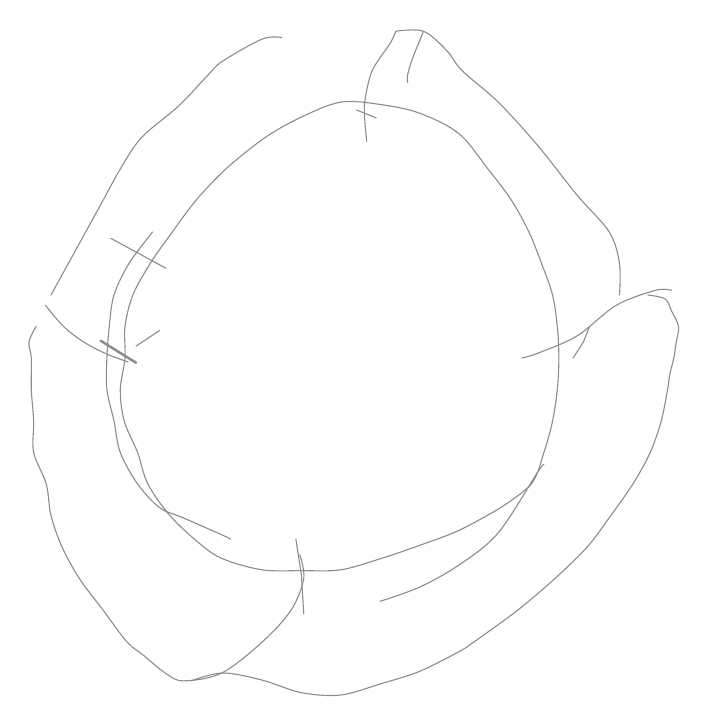
\begin{tikzpicture}[x=1mm,y=1mm,line cap=round,line join=round,font=\scriptsize]
\draw[pencil] plot[smooth, tension=0.55] coordinates {(70,-85.2) (74.2,-82) (75.8,-78) (76.9,-74) (77.5,-70) (77.7,-66) (77.5,-62) (76.9,-58) (75.5,-54) (73.9,-50) (71.7,-46) (68.7,-42) (65,-37.5) (60,-34.9) (55,-33.8) (50,-33.5) (45,-35.4) (40.4,-38) (35.4,-42) (31.6,-46) (28.6,-50) (25.8,-54) (23.6,-58) (22.6,-62) (22.6,-66) (22,-70) (22.5,-74) (24.2,-78) (25.5,-82) (28.3,-86) (32,-89.5) (35,-91.5) (40,-92.9) (45,-93) (50,-92.9) (55,-91.5) (60,-89.8) (65,-87.9) (70,-85.2)};
\draw[pencil] plot[smooth, tension=0.55] coordinates {(75.8,-79.5) (75,-80.5) (70,-88.2) (65,-92.3) (60,-95.1) (55,-96.9)};
\draw[pencil] plot[smooth, tension=0.55] coordinates {(26.1,-50) (23.1,-54) (21.2,-58) (20.6,-62) (20.3,-66) (20.3,-70) (21.2,-74) (22,-78) (24.2,-82) (27,-85) (30,-86.3) (35,-88.5) (36,-89)};
\draw[pencil] plot[smooth, tension=0.55] coordinates {(13.2,-58) (15.4,-54) (17.6,-50) (19.8,-46) (22,-42) (24.7,-38) (29.4,-34) (33.2,-30) (35,-28.3) (40,-25.5) (42.5,-25.3)};
\draw[pencil] plot[smooth, tension=0.55] coordinates {(53.3,-38.5) (53,-34) (53.8,-30) (54.9,-28) (56.3,-26) (57,-24.5)};
\draw[pencil] plot[smooth, tension=0.55] coordinates {(58.5,-31) (58.5,-30) (59.1,-28) (59.9,-26) (60.5,-24.5)};
\draw[pencil] plot[smooth, tension=0.55] coordinates {(57,-24.5) (60.5,-24.5) (63.5,-27) (65.4,-29.5) (70,-33.5) (75,-39) (80,-45.3) (84.1,-50) (85.4,-54) (85.4,-58)};
\draw[pencil] (52,-34.5) -- (54.5,-35.5);
\draw[pencil] plot[smooth, tension=0.55] coordinates {(73,-66) (75,-65.4) (80,-63.2) (85,-59.3) (90,-57.4) (92,-57.4)};
\draw[pencil] (79.5,-66) -- (80.8,-64) -- (81.6,-62);
\draw[pencil] plot[smooth, tension=0.55] coordinates {(89,-58) (91.2,-58.5) (92,-60) (92.9,-62) (92.6,-64) (92.3,-66) (91.8,-68) (91.5,-70) (90.7,-74) (89.3,-78) (87.1,-82) (84.3,-86) (81.3,-90) (77.2,-94) (72.5,-98) (67,-102) (65,-103.3) (60,-105.8) (55,-107.4) (50,-108.8) (45,-108.5) (40,-106.9) (35,-106) (31,-107)};
\draw[pencil] plot[smooth, tension=0.55] coordinates {(12.5,-59.3) (14.8,-62) (17.4,-64) (20.3,-65.5) (23,-66.5)};
\draw[pencil] plot[smooth, tension=0.55] coordinates {(11.3,-62) (10.4,-64) (10.7,-66) (10.7,-70) (11,-74) (11,-78) (12.6,-82) (13.2,-86) (14.6,-90) (16.8,-94) (19.8,-98) (22.8,-102) (25,-103.8) (27.7,-106) (30,-107) (34.9,-106) (40.1,-102) (43.7,-98) (45.3,-94) (44.8,-91)};
\draw[pencil] (44.3,-89) -- (45,-93.5) -- (45.3,-98.5);
\draw[pencil] (20.8,-50.8) -- (27.8,-54.6);
\draw[pencil,line width=0.9pt] (19.5,-63.8) -- (24,-66.6);
\draw[pencil] (24,-64.5) -- (27,-62.5);
\end{tikzpicture}
\end{document}
